\chapter{Artificial Neural Networks}

One of the most powerful methods to solve the face recognition problem are Artificial Neural Networks. 
A good definition of ANN, is given by Haykin [TODO] describing ANN as a parallel combination of simple  processing unit which can acquire knowledge from environment through a learning process and store the knowledge in its connections. The idea of Artificial Neural Network was inspired by biological neural networks (in particular the brain). 

\section{Biological background}
A neuron, in a biological sense, is a cell that carries and processes information - electric signal. The typical neuron is composed of cell body (perikarion) and two types of "branches": axons and dendrites. The cell body consists of plasma and a nucleus that holds information about hereditary traits. Each neuron receives an information from other neurons through the dendrites and transmits the processed information via axons. Axon - dendrites connection is called synapse. 

\begin{figure}[H]
\centering
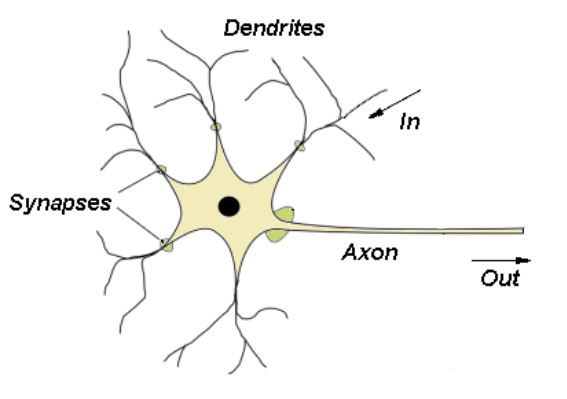
\includegraphics[scale=1]{neuron_schema.jpg}
\caption{Biological Neuron Schema}
\end{figure} 

The synapse's effectiveness can be adjusted by the signals passing through it so that the synapses can learn from the activities in which they participate. 

A typical person is capable of making complex perceptual decisions such as face recognition within a few hundred milliseconds. These decisions are made by a network of neurons whose operational speed is only a few milliseconds. This implies that the computations cannot take more than about 100 serial steps. This is knows as a hundred step rule: the brain runs parallel programs that are at most 100 steps long for such a tasks.

It can be deduced that the amount of information sent from one neuron to another is very small. Hence, the critical information is not transmitted directly, but captured and distributed in the neuron interconnections. 

That is also one of the features of Artificial Neural Networks. The system inspired by human brain are also hoped to posses some of the most desired brain's characteristics such as:

\begin{itemize}
\itemsep0em 
\item massive parallelism 
\item distributed representation and computation
\item learning ability 
\item adaptability
\item fault tolerance
\end{itemize}


\section{Artificial Neural Network architecture}

\subsection{Forward pass}

The smallest unit of computation in a neural network is the neuron, also called a node or unit. It receives an input from the other neurons or (in case of input neurons) from the external source. Each input has an associated weight, which is assigned proportionally to its relative importance to other inputs. The neuron produces the output by applying so called activation function to the weighted sum of its inputs.

\begin{figure}[H]
\centering
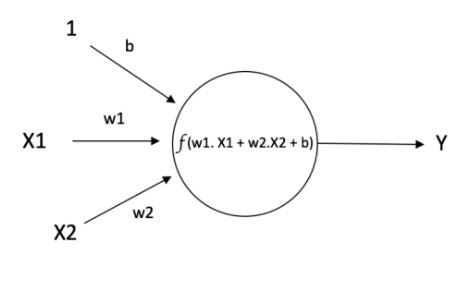
\includegraphics[scale=0.65]{single_neuron.jpg}
\caption{Single Neuron}
\end{figure} 


The activation function is applied in order to introduce non-linearity into the neurons' output. The choice of activation function is wide and it remains as an active area of research. The most commonly used activation functions are presented below: 

\begin{itemize}
\itemsep0em 
\item Sigmoid: squashes the input into the range between 0 and 1 
\begin{equation}
\sigma (x) = \frac{1}{1+\exp(-x)} 
\end{equation}
\item Hyperbolic tangent: squashes the input into the range between -1 and 1
\begin{equation}
tanh(x) = \frac{e^{x} - e^{-x}}{e^{x} + e^{-x}}
\end{equation}
\item Rectified Linear Unit (ReLU): It takes a real-valued input and thresholds it at zero
\begin{equation}
f(x) = max(0, x)
\end{equation}
\end{itemize}

According to the recent publications the ReLU function is believed to perform better than the other activation functions. Its simplicity reduces the computational complexity - it does not involve expensive operations such as exponentials. Another big advantage of ReLU is non-saturation of its gradient, which greatly accelerates the convergence of stochastic gradient descent compared to the sigmoid / tanh functions (TODO paper by Krizhevsky et 
al).

The general equation describing the neural network forward pass is given by:

\begin{equation}
\vec{o} = f(\vec{w} \cdot \vec{x} + b) 
\end{equation}

where $o$ is the output vector, $f$ is an activation function, $\vec{w}$ is a weights vector, $\vec{x}$ is a vector of layer input, $b$ is a bias.

\section{Backpropagation}

One of the main requirements for training this kind of algorithms is data. All learning algorithms use data in their training processes, but ANN require more than most.Given the data, there are various learning algorithms, from which gradient descent (backpropagation) is considered the most successful of all of them.


Backpropagation, also called gradient descent, is a common method for training a neural network. It is used for training Multilayer Perception Network as well as Convolutional Neural Network.

The basic idea of gradient descent method is to adjust the parameters of the neural networks in the way that the computed difference between predicted and expected values will be minimized. 

The choice of error functions (cost functions) is wide. One of the simplest approaches is to calculate the Euclidean distance between the predicted $o$ and expected $o'$ values: 

\begin{equation}
E_{1}(o,o') = \frac{||o-o'||^{2}}{2}
\end{equation}

The error can be also calculated using Mean Squared Error: 
\begin{equation}
E_{2}(o,o') = \frac{\sum_{k=1}^{K}(o_{i} - o'_{i})^2}{K}
\end{equation}
where $K$ is the size of output vector.

When using a neural network to perform classification and prediction, it is usually better to use cross-entropy error than classification error or mean squared error, due to the better convergence of the gradient.

The cross-entropy error function for multi-class output is defined as:

\begin{equation}
E_{3}(o, o') = -\sum_{i=1}^K o'_{i} \ln(o_{i})\end{equation} 


Since the goal of backpropagation is to minimize the error E, which depends on the network weights, we have to deal with all weights in the network one at a time.
To perform the backpropagation, the output of each unit from the forward pass must be stored. The gradients with respect to each parameter $w_{ij}$ is being calculated.

\begin{enumerate}
\itemsep0em
\item As a first step we calculate so-called errors $\delta_{i}^{(o)}$ for the output units:

\begin{equation}
\delta_{i}^{(o)} = \frac{\partial E}{\partial o_{i}} f'(z_{i})
\end{equation}

where $z_{i}$ is the input to the output layer.
\item We determine $\delta_{i}^{(l)}$ for all hidden layers in the network:

\begin{equation}
\delta_{i}^{(l)} = f'(z_{i}^{(l)}) \sum_{k=1}^{m^{(l+1)}} w_{i,k}^{(l+1)} \delta_{k}^{(l+1)}
\end{equation}
where $m^{(l)}$ is the number of units in layer $l$.
\item We calculate the derivative:
\begin{equation}
\frac{\partial E}{\partial w_{j,i}^{(l)}} = \delta_{j}^{(l)}y_{i}^{(l-1)}
\end{equation}
\item Once all partial derivatives have been computed, the gradient descent is performed by subtracting from each weight the increment:
\begin{equation}
\Delta w_{ij} = \lambda z_{j}^{(l-1)} \delta_{j}^{(l)}
\end{equation}

where $\lambda$ is a learning rate, which determines how fast the network coefficients change. 
\end{enumerate}

After choosing the initial weights of the network randomly, the backpropagation algorithm is used to compute the necessary corrections. The neural network training process can be decomposed in the following steps:

\begin{enumerate}
\itemsep0em 
\item Feed-forward pass
\item Backpropagation of each layer
\item Weight updates
\end{enumerate}
The algorithm is stopped when the value of the error function is sufficiently small.


\subsection{ANN topology}

The architecture of an artificial neural network defines how its several neurons are arranged, or placed, in relation to each other. In general an artificial neural network architecture can be divided into three parts (figure 6.2):

\begin{enumerate}
\itemsep0em 
\item Input layer - responsible for receiving normalized information, signals, features, or measurements from the user.
\item Hidden layer (or layers) - responsible for further information processing such as extracting patterns associated with the process. 
\item Output layer - responsible for producing and presenting the final network outputs, which result from the previous information processing.
\end{enumerate}

\begin{figure}[H]
\centering
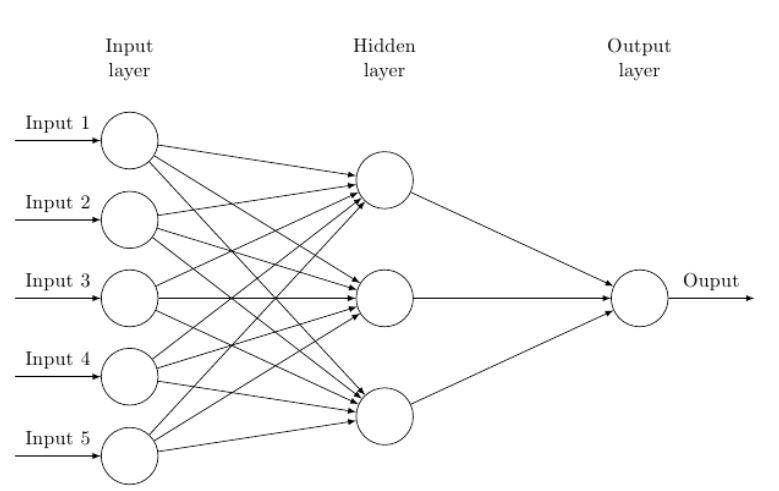
\includegraphics[scale=0.65]{ANN_schema.jpg}
\caption{Basic Artificial Neural Network Schema}
\end{figure} 

The presented ANN structure performs a feed-forward process. The connections only project forward, that is, neurons in a layer send the signal only to the subsequent layer. Furthermore, there are no connections between neurons in the same layer or between non-adjacent layers. 

There are plenty various configurations of feed-forward ANN, which can differ in the number of neurons in each layer as well as in the amount of layers. 

\begin{figure}[H]
\centering
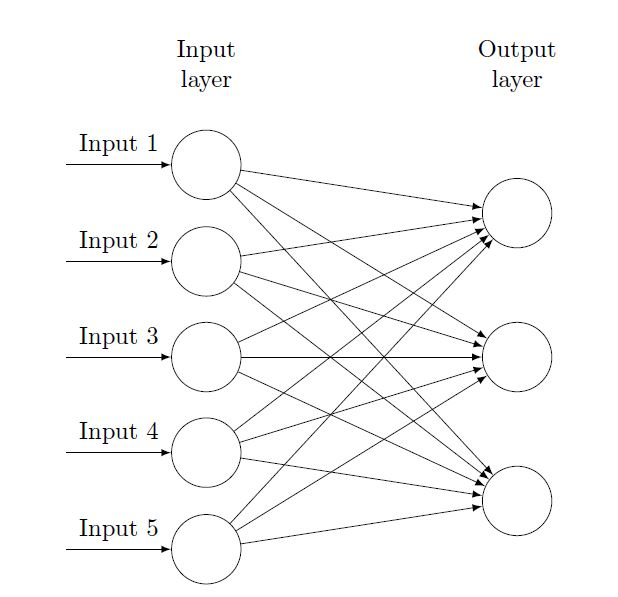
\includegraphics[scale=0.65]{single_ANN_schema.jpg}
\caption{Single-layer Artificial Neural Network Schema}
\end{figure} 

\begin{figure}[H]
\centering
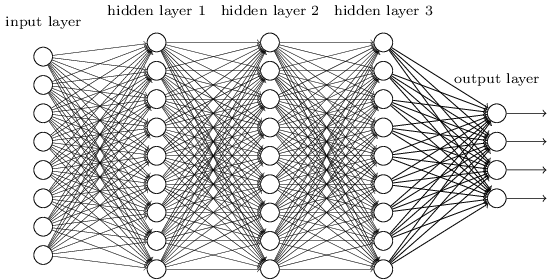
\includegraphics[scale=0.65]{img/neural_net.png}
\caption{Example of Deep Neural Network architecture}
\end{figure}

The neural network with more than one hidden layer is known as Deep Neural Network. (Figure 6.4). This type of ANN is suitable for processing very high-dimensional data, hence it seems to be a good choice for the facial recognition system design. 



